\documentclass[a4paper]{book}
\usepackage{makeidx}
\usepackage{graphicx}
\usepackage{multicol}
\usepackage{float}
\usepackage{listings}
\usepackage{color}
\usepackage{ifthen}
\usepackage[table]{xcolor}
\usepackage{textcomp}
\usepackage{alltt}
\usepackage{ifpdf}
\ifpdf
\usepackage[pdftex,
            pagebackref=true,
            colorlinks=true,
            linkcolor=blue,
            unicode
           ]{hyperref}
\else
\usepackage[ps2pdf,
            pagebackref=true,
            colorlinks=true,
            linkcolor=blue,
            unicode
           ]{hyperref}
\usepackage{pspicture}
\fi
\usepackage[utf8]{inputenc}
\usepackage{mathptmx}
\usepackage[scaled=.90]{helvet}
\usepackage{courier}
\usepackage{sectsty}
\usepackage[titles]{tocloft}
\usepackage{doxygen}
\lstset{language=C++,inputencoding=utf8,basicstyle=\footnotesize,breaklines=true,breakatwhitespace=true,tabsize=8,numbers=left }
\makeindex
\setcounter{tocdepth}{3}
\renewcommand{\footrulewidth}{0.4pt}
\renewcommand{\familydefault}{\sfdefault}
\begin{document}
\hypersetup{pageanchor=false}
\begin{titlepage}
\vspace*{7cm}
\begin{center}
{\Large test.c++ \\[1ex]\large 1 }\\
\vspace*{1cm}
{\large Generated by Doxygen 1.7.4}\\
\vspace*{0.5cm}
{\small Sun Apr 15 2012 19:34:52}\\
\end{center}
\end{titlepage}
\clearemptydoublepage
\pagenumbering{roman}
\tableofcontents
\clearemptydoublepage
\pagenumbering{arabic}
\hypersetup{pageanchor=true}
\chapter{File Index}
\section{File List}
Here is a list of all files with brief descriptions:\begin{DoxyCompactList}
\item\contentsline{section}{\hyperlink{test_8c_09_09}{test.c++} }{\pageref{test_8c_09_09}}{}
\end{DoxyCompactList}

\chapter{File Documentation}
\hypertarget{test_8c_09_09}{
\section{test.c++ File Reference}
\label{test_8c_09_09}\index{test.c++@{test.c++}}
}
{\ttfamily \#include $<$iostream.h$>$}\par
{\ttfamily \#include $<$ctype.h$>$}\par
Include dependency graph for test.c++:\nopagebreak
\begin{figure}[H]
\begin{center}
\leavevmode
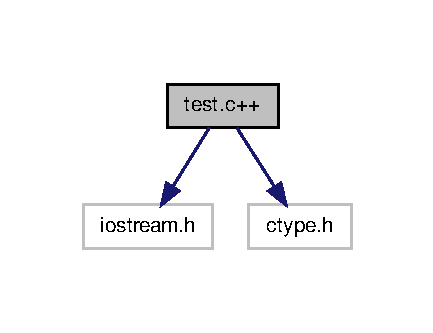
\includegraphics[width=208pt]{test_8c_09_09__incl}
\end{center}
\end{figure}
\subsection*{Functions}
\begin{DoxyCompactItemize}
\item 
void \hyperlink{test_8c_09_09_acdef7a1fd863a6d3770c1268cb06add3}{main} ()
\begin{DoxyCompactList}\small\item\em another lib to use toupper \end{DoxyCompactList}\end{DoxyCompactItemize}


\subsection{Function Documentation}
\hypertarget{test_8c_09_09_acdef7a1fd863a6d3770c1268cb06add3}{
\index{test.c++@{test.c++}!main@{main}}
\index{main@{main}!test.c++@{test.c++}}
\subsubsection[{main}]{\setlength{\rightskip}{0pt plus 5cm}void main (
\begin{DoxyParamCaption}
{}
\end{DoxyParamCaption}
)}}
\label{test_8c_09_09_acdef7a1fd863a6d3770c1268cb06add3}


another lib to use toupper 



moves char to lower case (like toupper)

puts 'grade' to a switch to cases below

inner barcket

break cuts exe at once

this points to the statement below

default 


\printindex
\end{document}
